\section{Methodology}
\label{section:algorithm}

Our framework, illustrated in Figure~\ref{fig:framework} and Algorithm~\ref{alg:meta_training}, extends the Hyp-RL 
formulation~\citep{jomaa2019hyp} along two axes: a derivative-informed state 
representation and a cross-dataset meta-training procedure. Both share the same 
LSTM policy and differ only in state features and training protocol.

\begin{figure}[H]
    \centering
    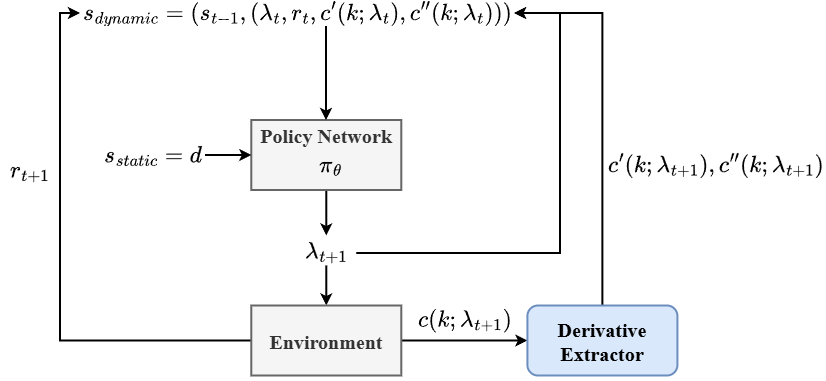
\includegraphics[width=0.8\textwidth]{framework.png}
    \caption{Framework}
    \label{fig:framework}
\end{figure}

\begin{algorithm}
\caption{CrossDataset-LC-DQN Meta-Training}
\label{alg:meta_training}
\begin{algorithmic}[1]
\REQUIRE Source datasets $\mathcal{D}$, Total episodes $E$, Training budget $T$
\STATE Initialize shared policy network $Q(s, a; \theta)$ and replay buffer $\mathcal{B}$
\FOR{episode $= 1$ \TO $E$}
    \STATE Sample a source dataset $D \sim \mathcal{D}$
    \STATE Extract static metadata descriptor $d$ from $D$
    \STATE Initialize LSTM hidden and cell states $(h_0, c_0)$ using $d$
    \STATE Initialize state sequence $s_0$ with $d$
    \FOR{$t = 1$ \TO $T$}
        \STATE Select hyperparameter configuration $a_t$ via $\epsilon$-greedy policy
        \STATE Evaluate $a_t$ on $D$ and obtain learning curve $c(k; a_t)$
        \STATE Extract curve features $s_{lc}$ (including derivative statistics) from $c(k; a_t)$
        \STATE Compute improvement reward $r_t$
        \STATE Update dynamic state $s_{t} = (s_{t-1}, (a_t, r_t, s_{lc}))$
        \STATE Store transition $(s_{t-1}, a_t, r_t, s_{t})$ in $\mathcal{B}$
        \STATE Update network parameters $\theta$ by sampling mini-batches from $\mathcal{B}$
        \IF{termination condition is met}
            \STATE \textbf{break}
        \ENDIF
    \ENDFOR
\ENDFOR
\end{algorithmic}
\end{algorithm}

\paragraph{Derivative-informed state.}
Rather than feeding the full derivative sequence $c'(k)$, $c''(k)$ into the 
network, we summarize each observed learning curve with five compact 
finite-difference statistics over its last 8 epochs: the final value, minimum, 
mean first difference (slope), mean second difference (curvature), and total 
improvement. These features are appended to each history row, increasing the 
input dimension by five. We refer to this variant as \textbf{CrossDataset-LC-DQN}, with 
\textbf{CrossDataset-HyperRL} denoting the ablation without curve features.

\paragraph{Dataset meta-features.}
We characterize each dataset using a 16-dimensional static descriptor $d \in \mathbb{R}^{16}$. This descriptor comprises structural and statistical meta-features extracted from the dataset, as detailed in Table \ref{tab:meta_features}. These 16 values are concatenated and $L_2$-normalized per dataset to form the static descriptor $d$. This descriptor is appended to every history row so that each per-step input is aware of the dataset's structural properties. Additionally, it is projected through two linear layers to initialize the LSTM hidden and cell states ($h_0, c_0$), priming the recurrent policy before any configuration is evaluated.

\begin{table}[htbp]
\centering
\caption{Extracted Dataset Meta-Features}
\label{tab:meta_features}
\begin{tabular}{ll}
\toprule
Number of Instances & Kurtosis Min \\
Log Number of Instances & Kurtosis Max \\
Number of Features & Kurtosis Mean \\
Log Number of Features & Kurtosis Standard Deviation \\
Data Set Dimensionality & Skewness Min \\
Log Data Set Dimensionality & Skewness Max \\
Inverse Data Set Dimensionality & Skewness Mean \\
Log Inverse Data Set Dimensionality & Skewness Standard Deviation \\
\bottomrule
\end{tabular}
\end{table}

\paragraph{Cross-dataset meta-training.}
We learn a single shared LSTM across source datasets via round-robin sampling: 
each meta-training episode samples one source dataset, runs a full HPO episode 
of length $T$, and updates the shared policy from a shared replay buffer. To 
stabilize learning across heterogeneous loss scales, we use an improvement 
reward $r_t = \max(0, -f_t + f_{t-1})$. After meta-training, the policy is frozen ($\varepsilon=0.01$) and evaluated on held-out target datasets, while non-meta baselines are reinitialized per target under the same budget.